\subsection{Revisione di Progettazione (RP)}
\subsubsection{Qualità di processo}
In questa sezione verranno analizzate le metriche e le valutazioni scaturite da esse.
\paragraph{Metriche dei processi}
\hspace{10cm}
\newline Verranno presentate solo le metriche dei processi ISO utilizzate fino ad ora.
Per gli esiti viene usata la stessa codifica del paragrafo precedente.
\begin{table}[!htbp]
	\centering
	\renewcommand{\arraystretch}{2} 
	\rowcolors{2}{gray!25}{white}
	\begin{tabular}{|l|p{2cm}|p{7cm}|l|}
		\rowcolor{orange!50}
		\hline
		\textbf{Processo} & \textbf{Valore ottenuto} & \textbf{Commento} & \textbf{Esito} \\
		\hline
		Schedule Variance & ~-7 giorni & Come si può notare dal diagramma di Gantt del \PdP sono stati raggiunti gli obiettivi con 7 giorni di anticipo, permettendoci di anticipare un po' il lavoro della prossima fase. & ~~X \\
		\hline
		Budget variance & ~~\EUR{ -765} & Avendo terminato in anticipo, siamo riusciti ad anticipare il lavoro della fase successiva, di conseguenza sono aumentate le ore di lavoro in questa fase. &  ~~X \\
		\hline
		{Indisponibilità servizi esterni} & ~~0 & Tutti i servizi esterni da noi usati non hanno avuto disservizi.  & ~~X\\
		\hline
		Rischi non calcolati & ~~2 & In questo periodo ci sono stati problemi di salute di alcuni membri, assieme all'aggiornamento di Grafana. Il tutto è presentato all'interno del \PdP & ~~X\\
		\hline
	\end{tabular}
	\caption{Metriche dei processi della fase di Progettazione Architetturale }
\end{table}
\clearpage
\paragraph{Code coverage}
\hspace{15cm}
\begin{figure}[!htbp]
	\centering
	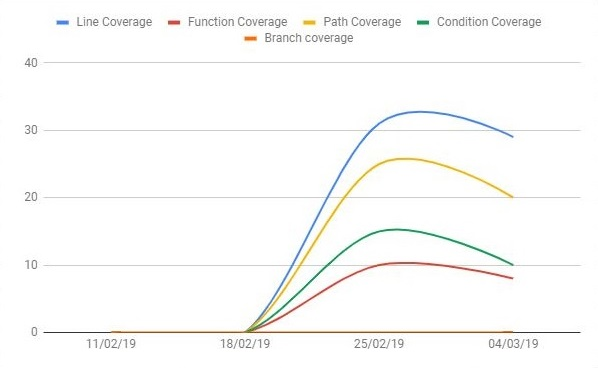
\includegraphics[scale=0.8]{CodeCoverageRP.JPG}
	\caption{Code coverage della fase di Progettazione Architetturale }
\end{figure}
\paragraph{Maturità macro-processi ISO }
\hspace{15cm}
\begin{figure}[!htbp]
	\centering
	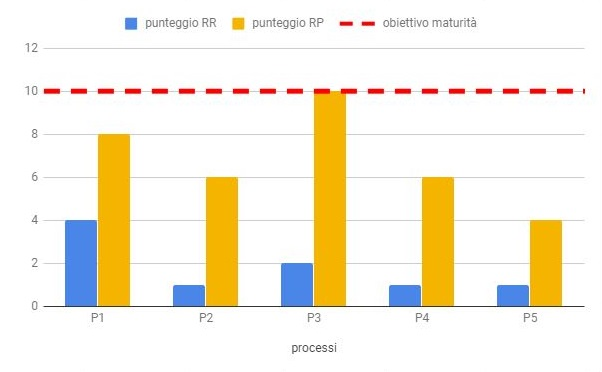
\includegraphics[scale=0.8]{MaturitaProcessiRP.JPG}
	\caption{Maturità macro-processi ISO 15504 della fase di Progettazione Architetturale }
\end{figure}
\begin{itemize}
	\item \textbf{P1:} processo gestito da automatismi, il gruppo ha acquisito una discreta familiarità, ma non è ancora sufficiente per considerarsi maturi;   
	\item \textbf{P2:} processo non ancora completamente funzionante perché i test non sono ancora stati sviluppati completamente né implementati;
	\item \textbf{P3:} processo completamente automatizzato e ormai maturo;
	\item \textbf{P4:} come per il processo 2, questo non è ancora stato del tutto istanziato a causa della mancanza dei test di verifica, sarà comunque completamente automatizzato;
	\item \textbf{P5:} processo sviluppato e implementato, ma non siamo riusciti ancora del tutto ad applicarlo.
\end{itemize}
\newpage
\paragraph{Build di Travis}
\hspace{15cm}
\begin{figure}[!htbp]
	\centering
	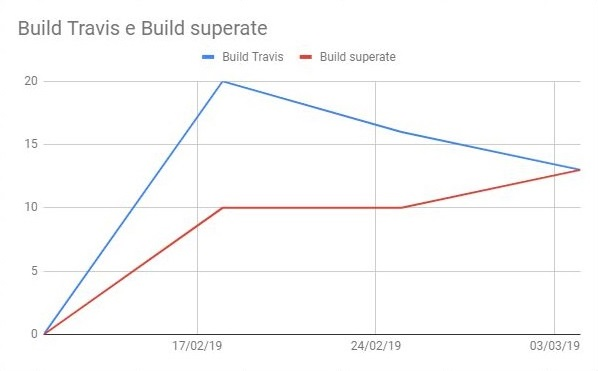
\includegraphics[scale=0.8]{BuildTravisRP.JPG}
	\caption{Media di Build Travis settimanale della fase di Progettazione Architetturale}
\end{figure}
    
\subsubsection{Qualità di prodotto}
In questa fase ci siamo concentrati sulla sistemazione dei documenti e sullo studio delle tecnologie che ci serviranno per la realizzazione del progetto facendo piccoli test di codice a se stante senza implementare i test.\\
Molti indici sul codice non sono nella zona di accettazione proprio a causa della mancanza dei test.\\
Le altre sono metriche prevalentemente sintattiche e pertanto sono da considerare con la dovuta cautela. \\
In particolari circostanze la valutazione automatica della leggibilità, se non tiene conto in alcun modo dei significati delle parole, può dare risultati inattendibili. \newpage
\paragraph{Gunning Fog index}
\hspace{15cm}
\begin{figure}[!htbp]
	\centering
	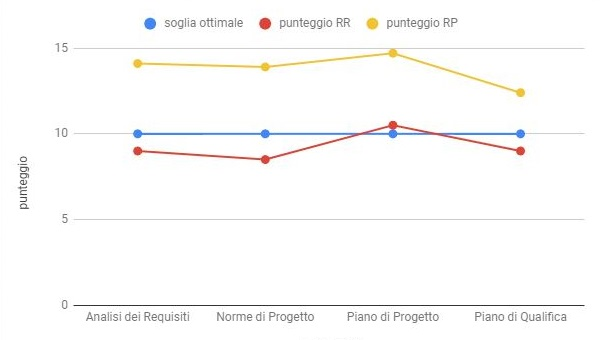
\includegraphics[scale=0.8]{GunningFogRP.JPG}
	\caption{Gunning Fog index della fase di Progettazione Architetturale }
\end{figure}
\clearpage
\paragraph{Simple Measure of Gobbledygook (SMOG) della fase di Progettazione Architetturale }
\hspace{15cm}
\begin{figure}[!htbp]
	\centering
	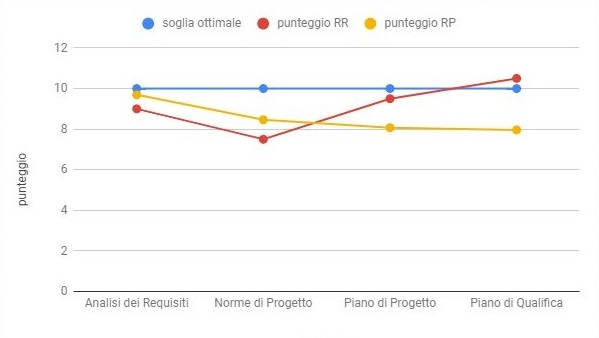
\includegraphics[scale=0.8]{SmogRP.JPG}
	\caption{SMOG}
\end{figure}
\newpage
\paragraph{Gulpease Index}
\hspace{15cm}
\begin{figure}[!htbp]
	\centering
	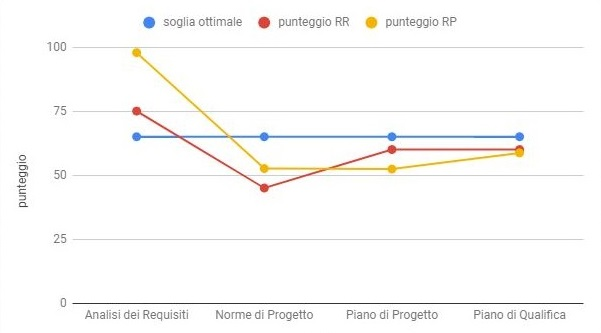
\includegraphics[scale=0.8]{GulpeaseRP.JPG}
	\caption{Gulpease index della fase di Progettazione Architetturale }
\end{figure}

\myparagraph{Errori sintattici}
 I verificatori hanno eliminato gli errori rimanenti presenti nei documenti, raggiungendo così il valore ottimale prefissato attraverso il software per il controllo ortografico presente in TexStudio. 